\documentclass[10pt]{article}
\usepackage[utf8]{inputenc}
\usepackage{amssymb}
\usepackage{amsmath}
\usepackage{amsthm}
\usepackage{graphicx} 
\usepackage{fullpage}
\usepackage[ruled,vlined,linesnumbered]{algorithm2e}
\usepackage{wrapfig}
\usepackage{float}
\usepackage{apacite}


\setlength{\parindent}{0em}  % set the indent of the paragraph
\setlength{\parskip}{0em} % set the space of the paragraph

\theoremstyle{definition}
\newtheorem{definition}{Definition}[section] % add the section number in front of the definition number
% \newtheorem*{definition}{Definition} % remove the index number of the definition

\title{Crash Data of Victoria state Exploration Project}
\author{Xianlin Feng \\  28847458 \\ xfen0007@student.monash.edu}
\date{\today}

\begin{document}
\maketitle

\section{Introduction}
\label{Introduction}
The road traffic accident is a threat to all people in their daily life. According to the WHO's statistics in 2018, road traffic accidents are the eighth of the top 10 causes of death, which is the only reason regarding injuries, and all the remaining reason are diseases. In worldwide, road injuries took 140 million lives in 2016, in which $74\%$ are men and boys \cite{WHO2016}. A serious situation happened in Victoria too. There were 58 lives lost because of the road accident every day in 2018 just in Victoria. This number increased to 88 since 7 April 2019. According to the TAC report, the lives lost of drivers takes nearly half ($48.2\%$) of the daily lives lost. The age of death concentrate in 30-69 years old. The most lives lost in rural roads($58\%$) \cite{TAC2019}. The analysis of past traffic accidents can provide a basis for future road construction, accident prevention, and accident rescue. The following three questions will be answered in this report:
\begin{enumerate}
	\item What is the trend in the last ten years?
	\item What is the main cause of road crashes in Victoria.
	\item What suggestion we can provide for the people in different areas.
\end{enumerate}
To answer those three questions, I will try to find one or more datasets, then perform data wrangling, data cleaning and data checking before data exploration. During the data exploration, I will use different statistic test methods and visualisation methods to explore the dataset and obtain insight. At last, I will provide some suggestions base on the result of the data exploration. The main structure of this report is as follow: the data wrangling will be processed in section \ref{dataWrangling}, then the data will be checking in section \ref{dataChecking}. The data exploration will be carried out in section \ref{dataExploration}, followed by conclusion in section \ref{conslusion} . In the last section, there will be a reflection of this assessment.\par


\section{Data Wrangling} 
\label{dataWrangling}
Data wrangling is a process to manipulate data to make the data directly usable for analysis. According to "2016 Data Science Salary Survey",  data scientists spend 53\% of their time for data cleaning and data wrangling \cite{dataWranglingTomar}. After data wrangling, the raw data is transformed into the data that can be analysed directly to generate insights and accurate results. Data wrangling is vital for a data science project, which not only improves the efficiency of data analysis but also reduces the error caused by incorrect data. In this section, I will divide the data wrangling process into the following small tasks base on the characteristics of the dataset:
\begin{enumerate}
	\item Introduce the dataset
	\item Filter the data
	\item Time series data handling	
	\item Drop missing or null values in the dataset
	\item deal with outliers or "illegal" values
\end{enumerate} \par


\subsection{the Dataset}
The dataset I found for this project named "CrashStats data", which could be downloaded on the Victoria government open data website: https://www.data.vic.gov.au. VicRoads provided the dataset for educational purposes, and it includes the crash data of time, location, conditions and so on since 2000. The dataset is consist of 12 tables, the main tables which will be used for this report are in the following list:
\begin{enumerate}
	\item \textbf{accident}:	contain the basic information about the accident, such as date, time, location, environment condition and severity.
	\item \textbf{vehicle}:	vehicle information, such as make, body type, year of manufacture, fuel type, vehicle capacity and so on.
	\item \textbf{person}:	personal details, such as age, sex, sitting position, passengers or driver, license state and so on.	
	\item \textbf{accident$\_$location}:	the location information of the accident.
	\item \textbf{road$\_$surface$\_$cond}:	the condition of the road: wet, dry, or icy.
	\item \textbf{atmospheric$\_$cond}:	weather condition: clear, wind, dust and so on.
	\item \textbf{accident$\_$node}:	more detailed location about the crash.
\end{enumerate}
Before the data wrangling and data cleaning, we need to understand the characteristics of each data table. For example, in the table of "accident", each accident has exact one record. However, as one accident may involve two or more people, one accident may have two or more records in the table "person". The same situation happens in table "vehicle", "accident$\_$event" and other tables too, this is another reason why this dataset separate to 12 data tables. Due to this reason, when we process data wrangling, data cleaning, or data exploration, extra care should be paid with multiple records for one accident. \par

\subsection{Time series data handling}
In the original dataset, the time information is stored in the format \text{"\textbf{hh.mm.ss}"}, which is not the common time format, so that I changed them to the format \text{"\textbf{hh:mm:ss}"} first. This step could easily perform in \textbf{Microsoft Excel} by just replacing every "." by ":". Then, the date and time information is separated into two columns, which is not very friendly to Tableau Public, so we need to combine them first. In order to complete this task, I need to insert a new column "\textbf{dateTime}" and in the cell "D2" use an Excel formulation:
\begin{center}
    \text{"\textbf{TEXT(B2,"d\/mm\/yyyy")\&" "\&TEXT(C2,"hh:mm:ss"})"}
\end{center}
This formulation could combine the date information in cell "B2" and time information in cell "C2" without lose any information. By applying this formulation to all rows, The new column could contain both date and time information could be generated.\par

\subsection{Filter data and Joint tables}	
The data of 2019 and before 2009 will not be considered in this report, so that, before we perform any data checking and data analysis, they need to be filtered. In the table "ACCIDENT", this step could easily be done in Tableau Public, since we have generated the new column named “DateTime". Then select data with speed zone under 120, and most analysis will base on the records which "NO$\_$PERSONS$\_$KILLED" is greater than 0. For the other tables, as the date information is only stored in the "ACCIDENT" table, this action could be more complicated, but every record in other tables contains "accident$\_$ID" field. So, an inner join is essential for each table and table "ACCIDENT". \par

\subsection{Identify key attributes}
\label{IdentifyKeyAttributes}
Another critical step after selecting data is to identify key attributes. Each data record contains lots of information related to the accident. However, some of them are not related to our project. So, select the useful data and information will help us for data checking and data analysis. Then data checking and correcting will be performed for the key attributes.\par

\section{Data Checking}
\label{dataChecking}
Tableau Public is a powerful tool for data wrangling, as well as data checking. In this section, I will demonstrate the foremost step I performed for data checking. More specific, checking the critical attributes of each table base on the property of the attribute.\par

\subsection{Check geographic data}
In the table "NODE", the attributes "lat" and "long" indicate the latitude and longitude coordinates for each accident. The attribute "Postcode$\_$No" demonstrate the suburb information. To check the attributes of "lat", "long" and "Postcode", just put them in the Tableau Public map, the result shows no record is outside Victoria state. So the geographic data is considered of complete and consist.\par

\subsection{Check duplicate record}
Eliminate duplicate records is important for data analysis. To complete this task, I used Tableau Public to identify the duplicate records in the key attributes. For example, for the "ACCIDENT$\_$No" in the table "ACCIDENT". The following command will calculate the time of one record appears in the field:\text{"\{fixed[Accident$\_$No:SUM([Number of Records])\}"}.
The result shows there is no duplicate records in "ACCIDENT$\_$No" attributes.\par

\subsection{Check the missing value}
\vspace{-12pt}
\begin{minipage}{\linewidth}
  	\centering
  	\begin{minipage}{0.53\linewidth}
		In Tableau Public, we can identify the missing value by summarise the table or each filed. The picture on the right shows the missing value of attribute "Road Type" in table "ACCIDENT$\_$LOCATION". As it showing in figure \ref{fig:identifyMissingValue}, there are 2964 missing value for attribute "Road Type", but the missing values are not critical for the data analysis, so that I just ignore them. Another method to deal with missing value is replacing the missing value with another value, such as 0. this could be done with function \textit{ZN()}.  \par
  \end{minipage}
  \hspace{0.03\linewidth}
  \begin{minipage}{0.4\linewidth}
        \begin{figure}[H]
     	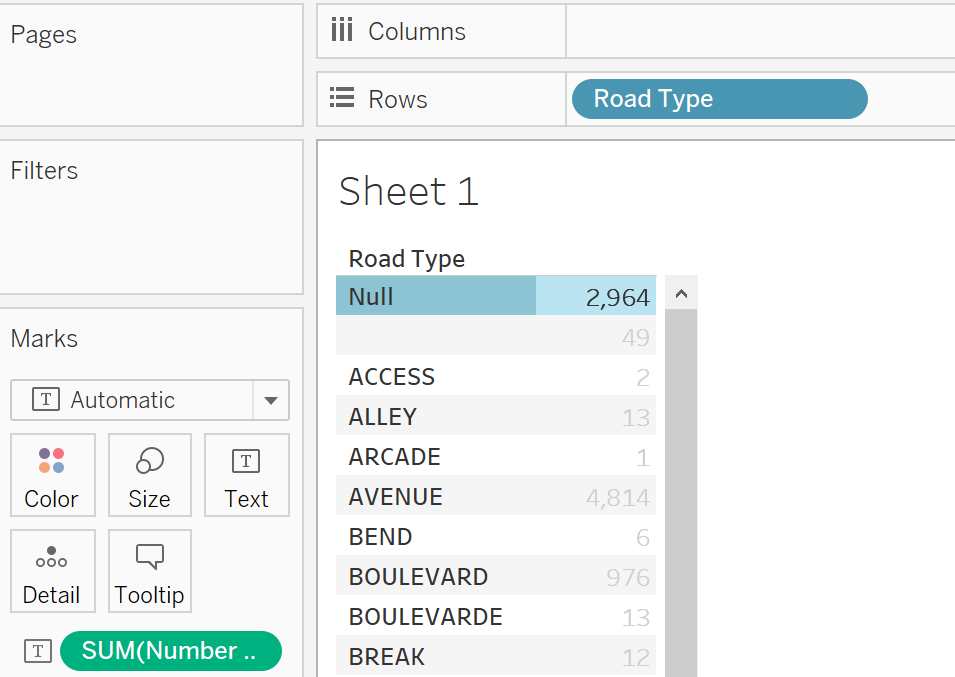
\includegraphics[width=\linewidth]{images/IdentifyMissingValue.png}
        \caption{Identify missing value}
        \label{fig:identifyMissingValue}
        \end{figure}
    \end{minipage}\\
    \vspace{12pt}
\end{minipage}\\ 

\subsection{Check outlier}
To check outlier in the field, we should identify the range first. For example, when checking the data range of the attribute "Node$\_$ID" in both table "ACCIDENT" and table "NODE" in Tableau Public, Two range could be found: $[4,\,342850]$ and $[-10,\,342850]$. Then I check the meta-data on the website of VicRoads. For the attribute of "Node$\_$ID", it explains that "The node id of the accident. It starts with 1 and incremented by one when a new accident location is identified" \cite{MetaData}. Therefore, the values blew 1 in the table "ACCIDENT" are outliers, and should not be used for analysis and exploration. Since the correct node id information is not known, the node id information cannot be used for analysing. Fortunately, the table "NODE" contains both accident information and node-id information, and it will be used in further data exploration. \par

\section{Data Exploration}
\label{dataExploration}
After data wrangling, cleaning, and checking, we have a clean and well-formatted dataset to analysis. In this section, I will perform data exploration and data analysis with Tableau Public and R. To answer the three questions proposed in section \ref{Introduction}, different statistical methods and visualisation methods will be used. I will mainly focus on traffic crashes which cause life loses. \par

\subsection{Trend of road crashes}
\begin{minipage}{\linewidth}
  	\centering
  	\begin{minipage}{0.48\linewidth}
     \begin{figure}[H]
              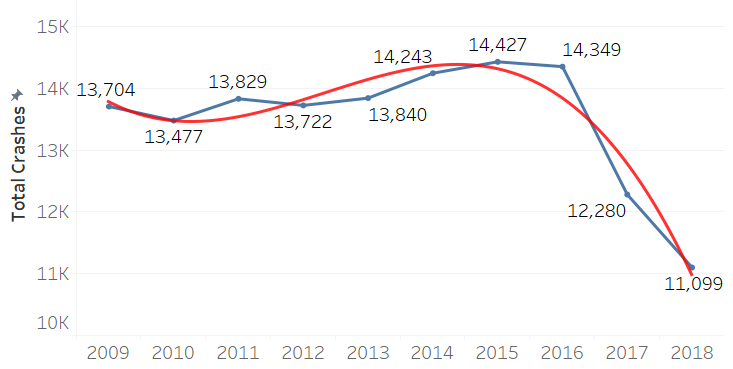
\includegraphics[width=\linewidth]{images/totalCrashOverYears.png}
              \caption{total crashes over 10 years}
              \label{fig:TrendYears}
    \end{figure}
  \end{minipage}
  \hspace{0.01\linewidth}
  \begin{minipage}{0.48\linewidth}
        \begin{figure}[H]
     	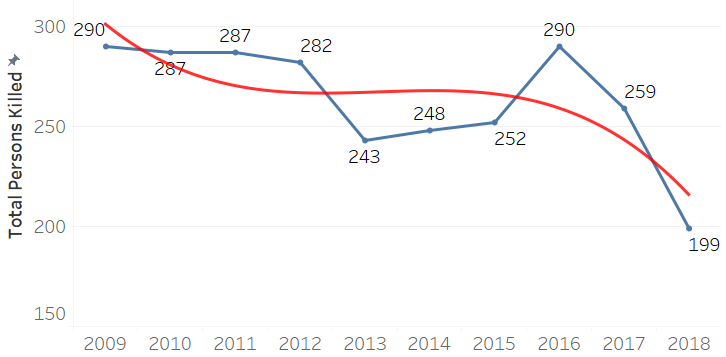
\includegraphics[width=\linewidth]{images/totalKilledOverYears.png}
        \caption{Total person killed over 10 years}
        \label{fig:TrendKillYears}
        \end{figure}
    \end{minipage}\\
    \vspace{12pt}
\end{minipage}\\
The figure \ref{fig:TrendYears} indicate that between 2010 and 2016, the total number of road crash increase slowly, but the number decreased rapidly in the year 2017 and 2018. A similar situation could also found in figure \ref{fig:TrendKillYears} in 2017 and 2018, which is a significant improve compare to those years from 2009 to 2016. \par

Every person with a driver license knows that more accidents happened on Friday, as well as the rush hours in the morning and afternoon. So that, to save the paper, I will skip those analyses, but move on to the reasons for the accidents. First, the analysis of different types of accident.  \par

\begin{figure}[H] % H means 	set the figure between the text.
	\centering
	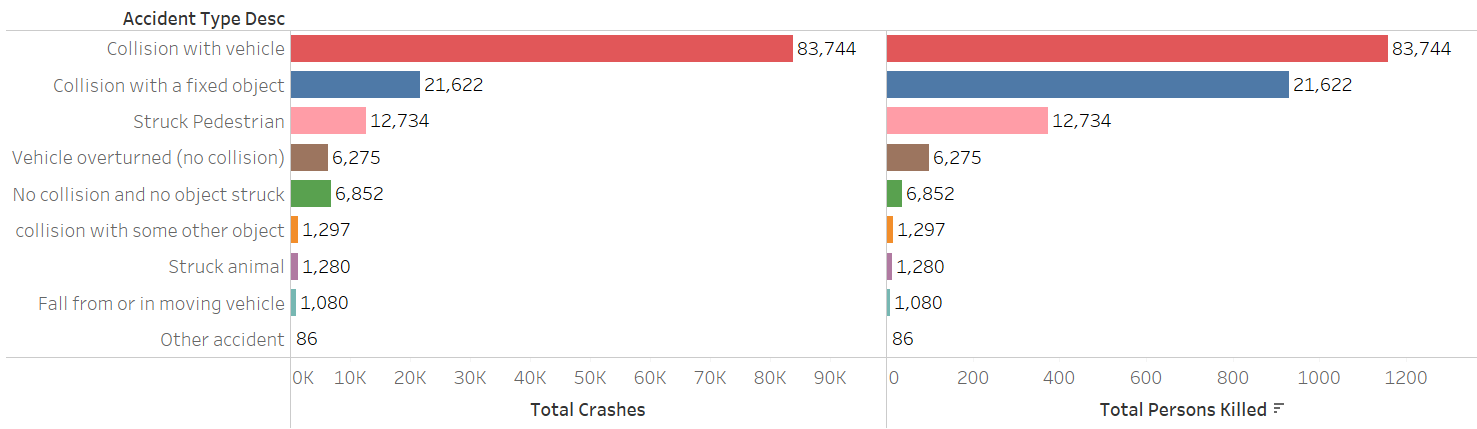
\includegraphics[width=\linewidth]{images/accidentType.png}
	\caption{Total crashes and person killed by different accident type}
	\label{fig:accidentType}
\end{figure}
According to figure \ref{fig:accidentType}, most of the accidents and life loses are caused by vehicles collision. However, collisions with fixed objects accounted for only 16.02$\%$ of the total number of accidents but accounted for 35.27$\%$ of all deaths in the dataset. \par 

\begin{minipage}{\linewidth}
  	%\vspace{-12pt}
  	\centering
  	\begin{minipage}{0.3\linewidth}
	The figure \ref{fig:accidentTypeTrend} shows that the trends of life lose for the top three accident types are decrease over the ten years. The peak record appeared in 2016, then drop rapidly in the last two years.
  \end{minipage}
  \hspace{0.01\linewidth}
  \begin{minipage}{0.66\linewidth}
     \begin{figure}[H]
              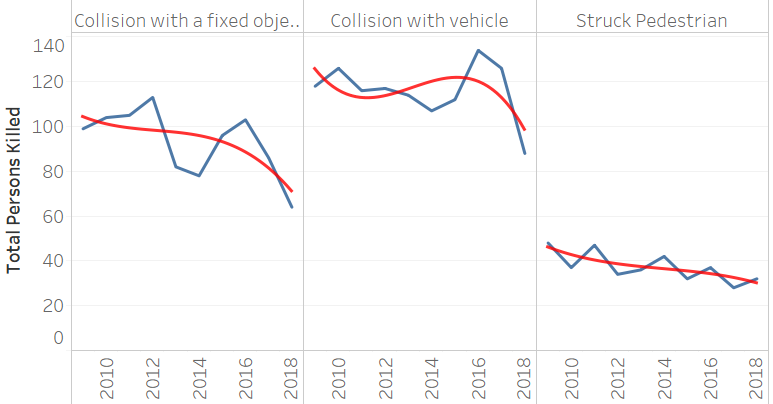
\includegraphics[width=\linewidth]{images/accidentTypeTrend.png}
              \caption{Trends of top 3 accident types}
              \label{fig:accidentTypeTrend}
    \end{figure}
    \end{minipage}
\end{minipage}
\vspace{12pt}\\
From the above, the statistics test indicate that not only the number of accidents but also the number of people get killed are decreased in the past ten years. To save space, more analysis details will not be shown. Instead, I will focus on the analysis of the cause of the accident, mainly on the accidents that caused the death of a person.

\subsection{main cause of road crashes in Victoria}
\label{main_cause}
In this section, more data exploration will be performed to find the leading cause of the person get killed in an accident in Victoria state, such as light condition, atmosphere condition, different accident type at the different road surface and so on. \par

First of all, to perform data analysis base on geographic information, the table "ACCIDENT" and the table "NODE" need to be joined together. An inner join base on the attribute of "Accident$\_$ID" could is the most reasonable choice for this task, because both tables use this attribute as their identity key.\par

\begin{minipage}{\linewidth}
  	\centering
  \begin{minipage}{0.59\linewidth}
	\begin{figure}[H]
            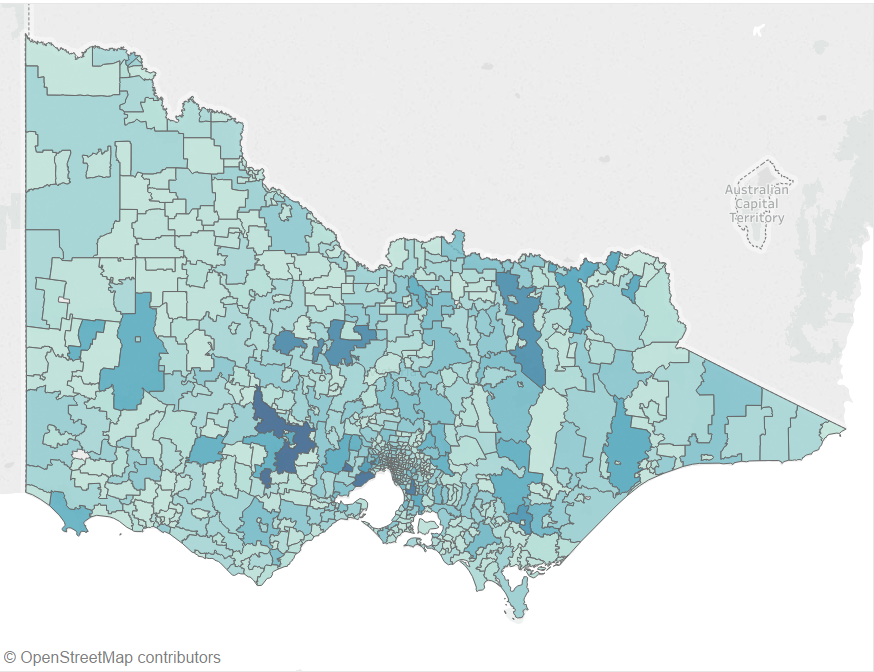
\includegraphics[width=\linewidth]{images/mapTotal.png}
			\caption{Total live loses in each suburb}
			\label{fig:mapTotal}
    \end{figure}
  \end{minipage}
  \hspace{0.0\linewidth}
  \begin{minipage}{0.39\linewidth}
     It is clearly shown in figure \ref{fig:mapTotal}, that \textbf{Bendigo}, \textbf{Cocoroc} and \textbf{Bangholme} take the top 3 number of life loses amount all suburbs in Victoria state. 
     \end{minipage}\\
\end{minipage}\\
\vspace{8pt}


\begin{minipage}{\linewidth}
  	\centering
  \begin{minipage}{0.49\linewidth}
	\begin{figure}[H]
            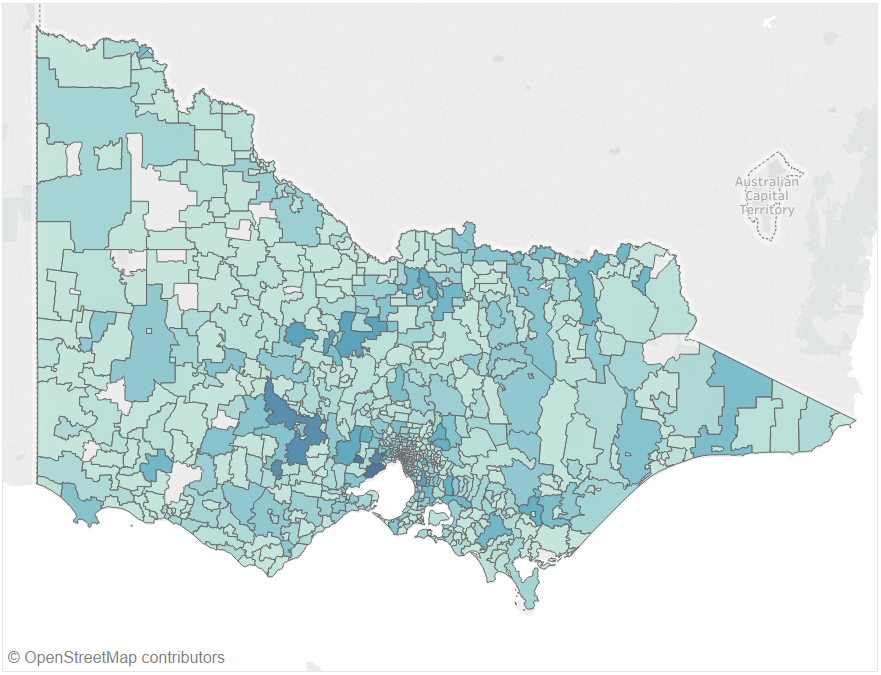
\includegraphics[width=\linewidth]{images/mapTypeVehicle.png}
			\caption{Total person killed by vehicles collision }
			\label{fig:mapTypeVehicle}
    \end{figure}
  \end{minipage}
  \hspace{0.0\linewidth}
  \begin{minipage}{0.49\linewidth}
     \begin{figure}[H]
            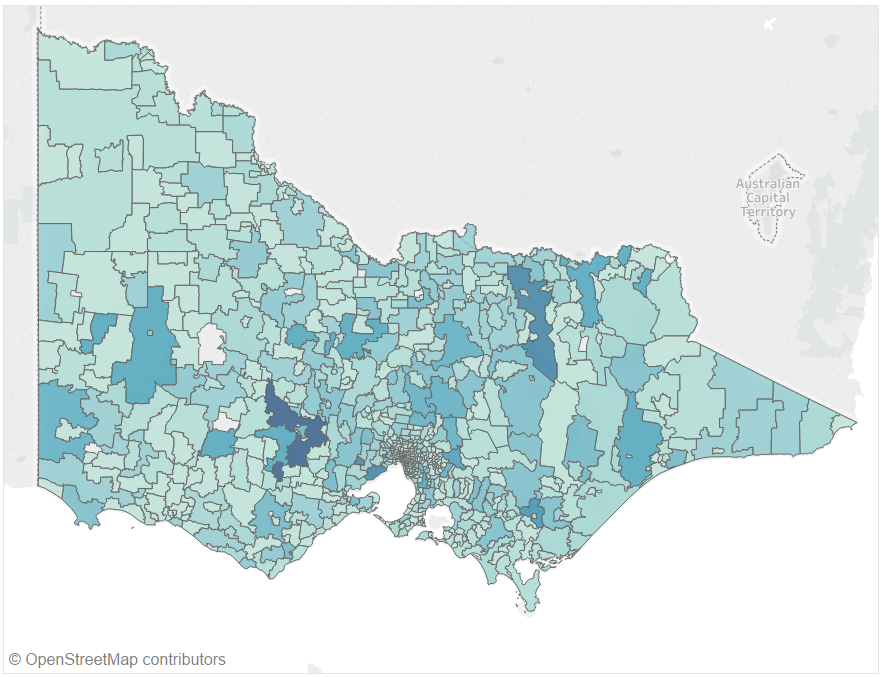
\includegraphics[width=\linewidth]{images/mapTypeObj.png}
			\caption{Total person killed by collision with a fixed object}
			\label{fig:mapTypeObj}
    \end{figure}
    \end{minipage}
\end{minipage}\\
\vspace{12pt}\\
As we can see from figure \ref{fig:mapTypeObj}, the suburb with postcode 3552 (\textbf{BENDIGO}) always have the most number of the person killed for the top 2 accident types.\par

\begin{minipage}{\linewidth}
  	\centering
  \begin{minipage}{0.49\linewidth}
	\begin{figure}[H]
            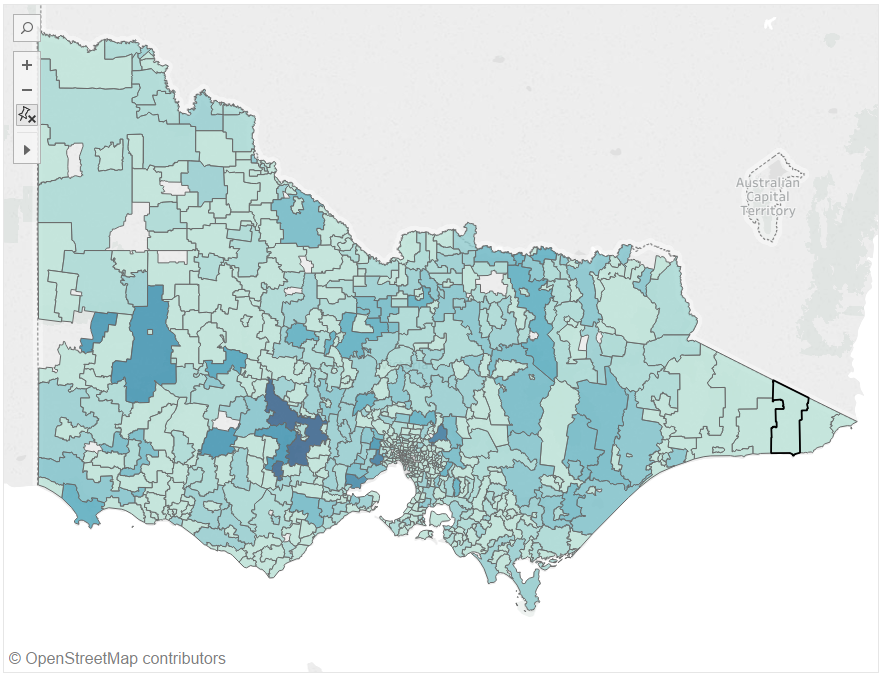
\includegraphics[width=\linewidth]{images/darkNoLight.png}
			\caption{Dark street with NO light }
			\label{fig:darkStreetNoLight}
    \end{figure}
  \end{minipage}
  \hspace{0.0\linewidth}
  \begin{minipage}{0.49\linewidth}
     \begin{figure}[H]
            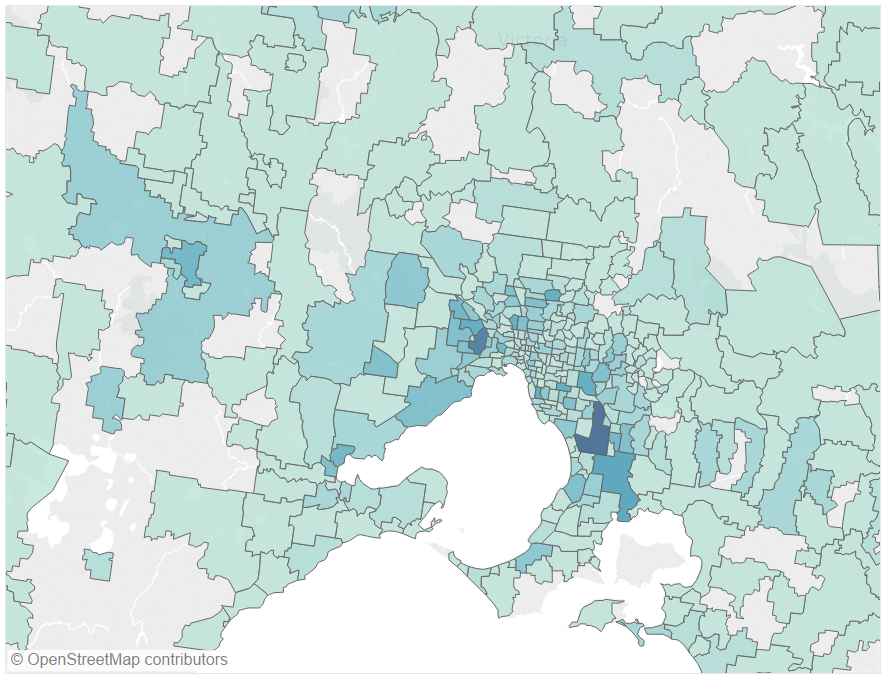
\includegraphics[width=\linewidth]{images/darkLightON.png}
			\caption{Dark street with light ON}
			\label{fig:darkStreetLightOn}
    \end{figure}
    \end{minipage}
\end{minipage}\\
\vspace{12pt}\\
The figure \ref{fig:darkStreetNoLight} indicates in the dark street the suburb with postcode 3552 (\textbf{BENDIGO}) got 15 people killed by the car accident, which is the highest record amount all. And figure \ref{fig:darkStreetLightOn} shows that the suburb of postcode 3175 (\textbf{BANGHOLME}) had 16 people killed. This result also reflects the construction of community street lights in different suburbs. \par

\begin{figure}[H] % H means 	set the figure between the text.
	\centering
	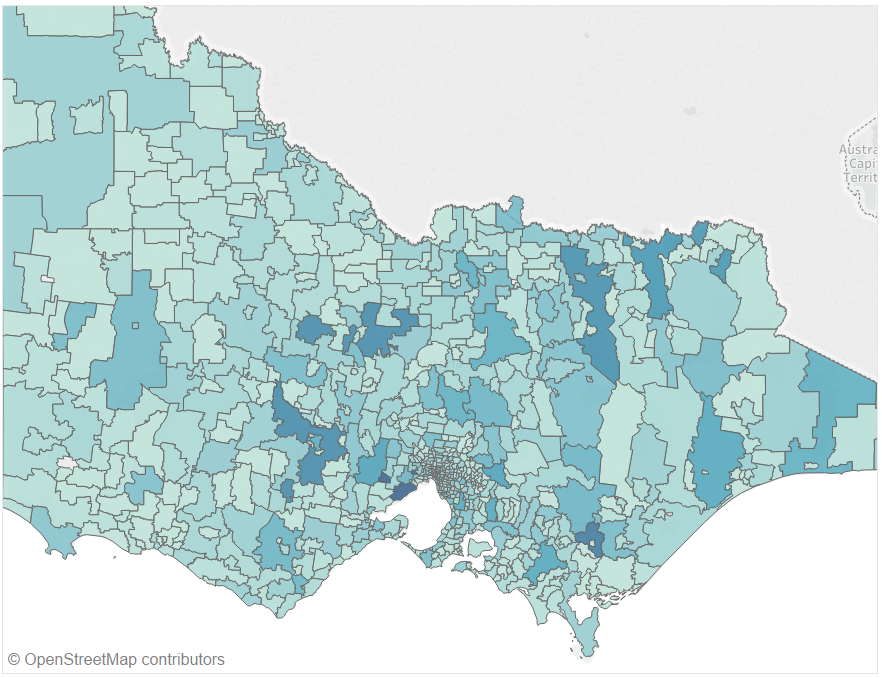
\includegraphics[width=0.7\linewidth]{images/day.png}
	\caption{No.person killed in daytime}
	\label{fig:day}
\end{figure}
The statistic in figure \ref{fig:day} illustrates that in the middle and north-east Victoria state occurred more deadly accident than other places. Unfortunately, one more time, the suburb of postcode 3552 still in the list of top risk suburbs.\par

\begin{minipage}{\linewidth}
  	\centering
  \begin{minipage}{0.45\linewidth}
	\begin{figure}[H]
		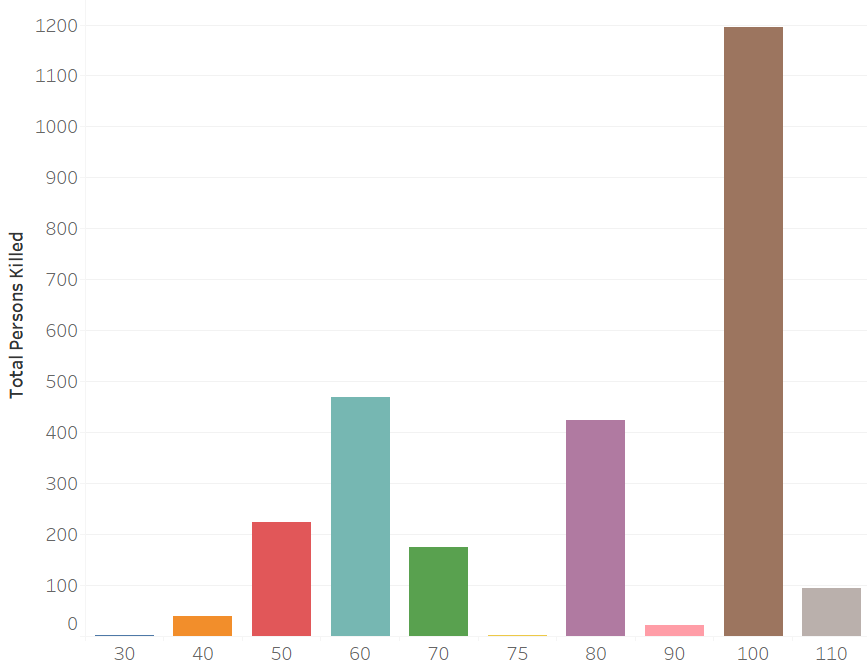
\includegraphics[width=\linewidth]{images/speedZone.png}
		\caption{Total life loses in each speed zone}
		\label{fig:speed}
    \end{figure}
  \end{minipage}
  \hspace{0.0\linewidth}
  \begin{minipage}{0.53\linewidth}
     \begin{figure}[H]
            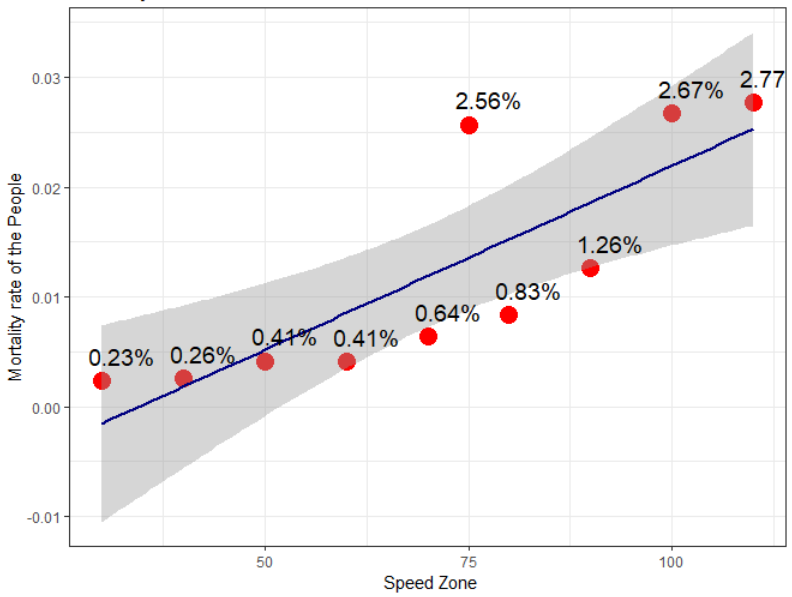
\includegraphics[width=\linewidth]{images/speedKillRateOfPeople.png}
				{\caption{Percentage of people get killed in each speed zone}}
			\label{fig:percentSpeedKills}
    \end{figure}
    \end{minipage}
\end{minipage}\\
\vspace{12pt}\\
From figure \ref{fig:speed} and figure \ref{fig:percentSpeedKills}, we could see that with the speed zone increase,  people can easier lose their life in a car accident. Besides, most of life loses appeared in the speed zone of 100. The same result could be found in the accidents which are in the atmospheric condition is "\textbf{strong winds}", and surface condition are "\textbf{Dry, Wet, Muddy}". The analysis process is similar to the analysis of "Speed Zone", to save the paper, the detailed analysis process will not be shown in the report. Now let us move on to the cluster. \par

\begin{minipage}{\linewidth}
  	\centering
  \begin{minipage}{0.49\linewidth}
	\begin{figure}[H]
		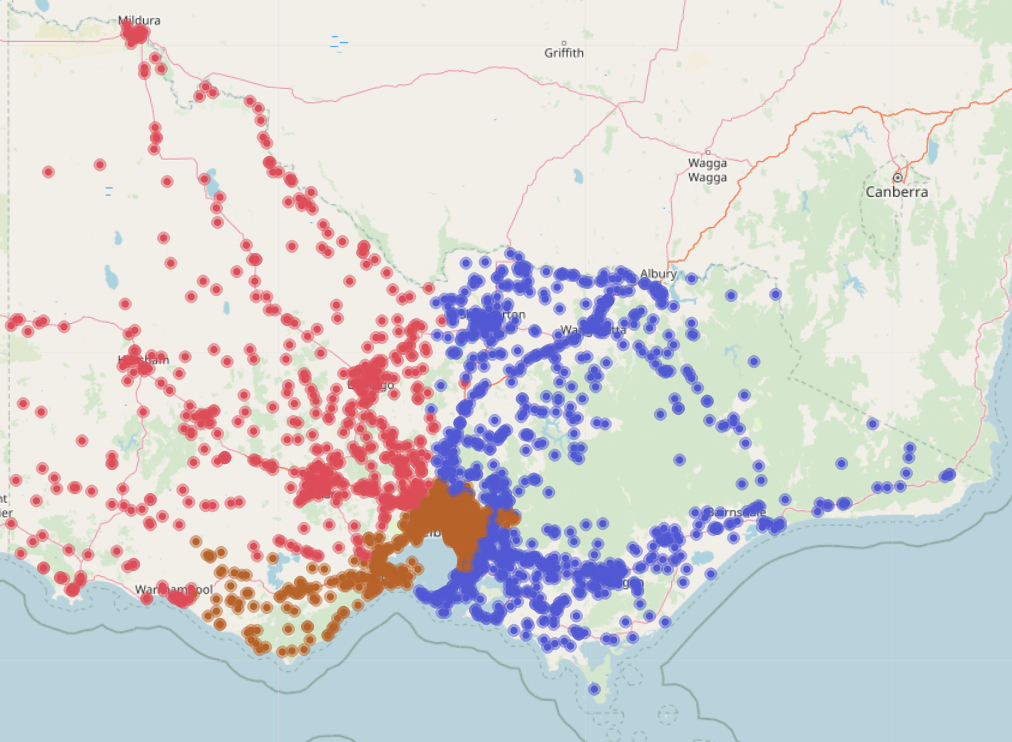
\includegraphics[width=\linewidth]{images/cluster3.png}
		\caption{Clustering with postcode}
		\label{fig:clusterWithPostcode}
    \end{figure}
  \end{minipage}
  \hspace{0.0\linewidth}
  \begin{minipage}{0.49\linewidth}
     \begin{figure}[H]
            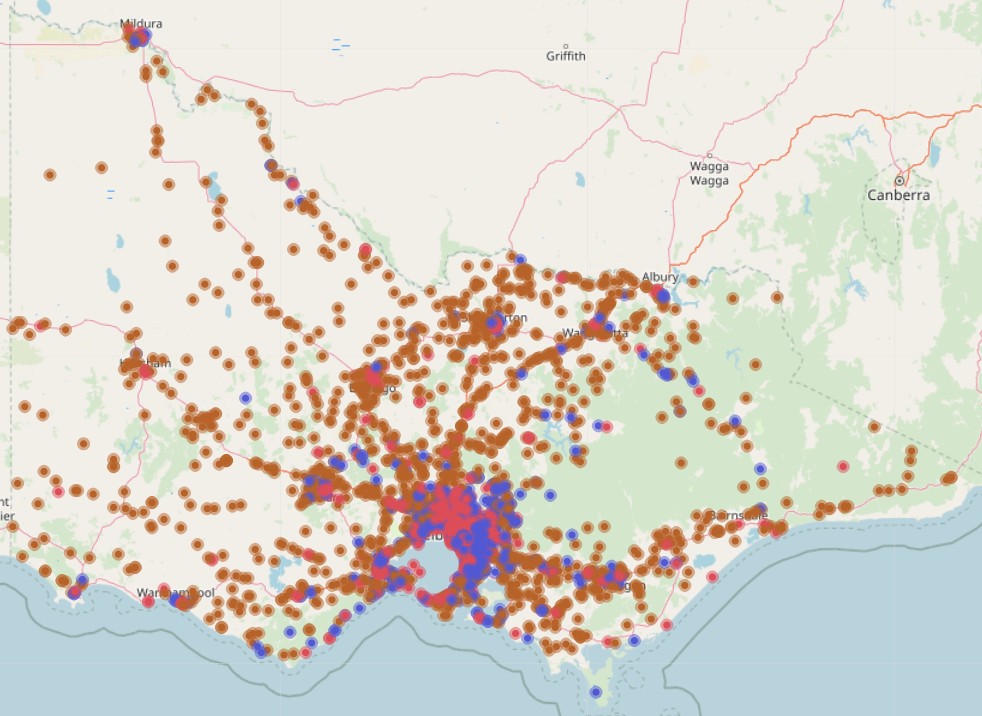
\includegraphics[width=\linewidth]{images/cluster3_NoPostcode.png}
				{\caption{Clustering without postcode}}
			\label{fig:cluster3}
    \end{figure}
    \end{minipage}
\end{minipage}\\
\vspace{12pt}\\
I use R to cluster the dataset, first select the data with the year of 2009 - 2018, the number of people killed is greater than zero, speed zone is less than 120. Afterwards, select the clustering attributes: accident type, light condition, surface condition, and atmospheric conditions. Then the dataset is clustered into 3 clusters. The figure \ref{fig:clusterWithPostcode} shows that if we consider postcode as a clustering attribute, each cluster is classified by region. If the postcode is not considered, new clusters are classified by geographic location: near the Melbourne city and outside the city. By analysis of the cluster, I found most of the accidents outside the Melbourne city are: 
\begin{itemize}
	\item Collision with a fixed object in the day time
	\item In the speed zone of 100
	\item On the dry road surface of a clear day
\end{itemize}

\begin{minipage}{\linewidth}
  	\centering
  \begin{minipage}{0.49\linewidth}
	\begin{figure}[H]
		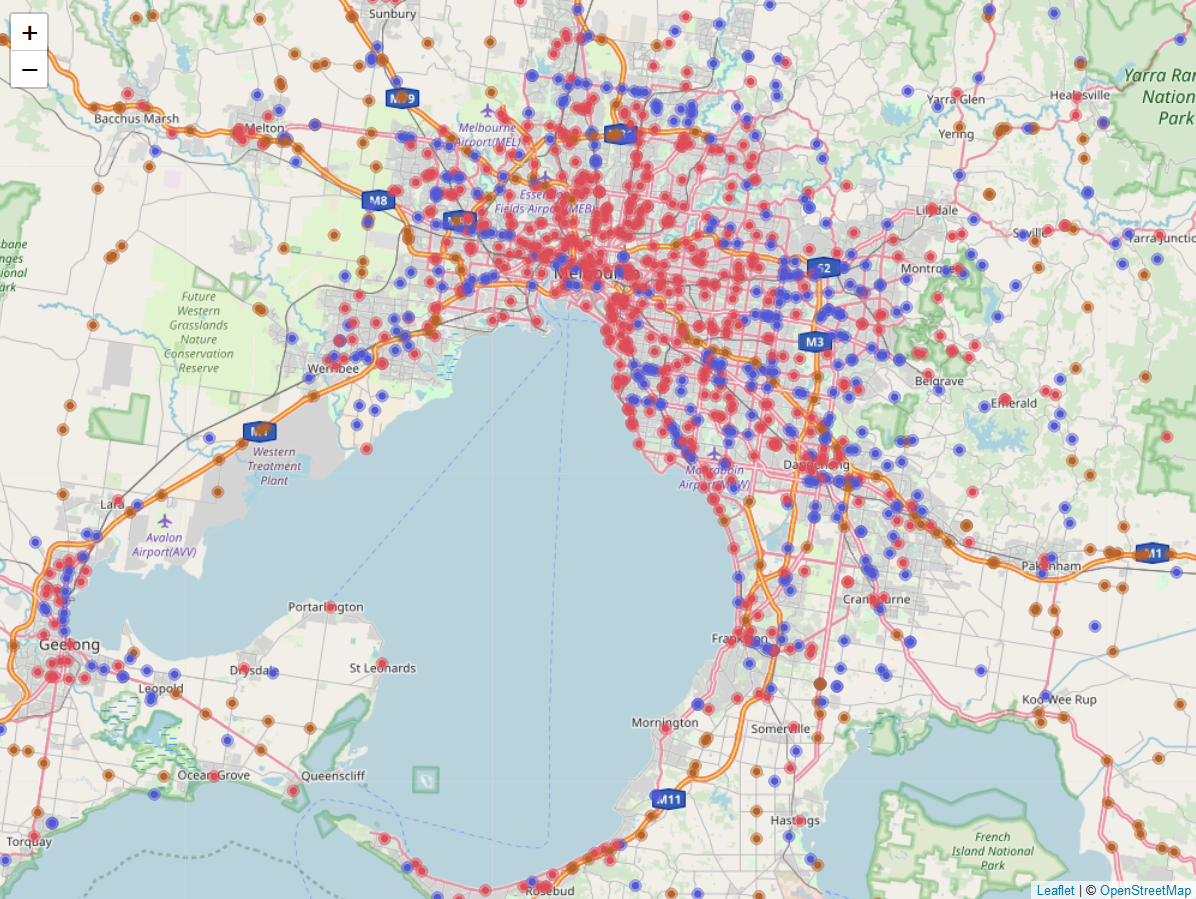
\includegraphics[width=\linewidth]{images/cluster3_NoPostcode_CBD.png}
		\caption{Clustering in Melbourne CBD}
		\label{fig:ClusterCBD}
    \end{figure}
  \end{minipage}
  \hspace{0.0\linewidth}
  \begin{minipage}{0.49\linewidth}
     The figure \ref{fig:ClusterCBD} shows that the cluster type is highly consistent near the CBD of the Melbourne city. The analysis shows that most accidents which caused people killed happened in the speed zone of 60 where the vehicles collide with another one.
    \end{minipage}
\end{minipage}\\
\vspace{12pt}\\

\begin{minipage}{\linewidth}
  	\centering
  \begin{minipage}{0.49\linewidth}
     If we extract text words from "Accident.Type.Desc", "Day.Week.Description", "Day.Week.Description", "Light.Condition.Desc", "Surface.Cond.Desc" and "Atmosph.Cond.Desc" from the filtered dataset, and perform text analysis and visualisation, the result is shown in figure \ref{fig:wordcloud} on the right.
  \end{minipage}
  \hspace{0.0\linewidth}
  \begin{minipage}{0.49\linewidth}
     \begin{figure}[H]
            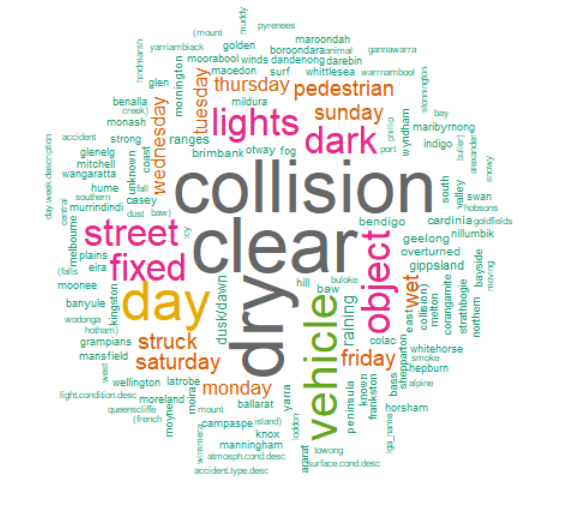
\includegraphics[width=\linewidth]{images/wordCloud.png}
				{\caption{Word Cloud of deadly accidents}}
			\label{fig:wordcloud}
    \end{figure}
    \end{minipage}
\end{minipage}\\


\section{Conclusion}
\label{conslusion}
According to the analyses above, the following recommendations can be provided for the drivers and local councils in Victoria state:
\begin{itemize}
    \item Bendigo, Cocoroc and Bangholme are the top 3 suburbs of people killed in accidents. Be more careful when driving through those suburbs. 
    \item Compared to other suburbs, Bendigo has more number of people killed in various statistics, and the local council need to do more analysis and try to make some improvements.
    \item Collision with a fixed object is more deadly compared to other accident types.
    \item Strong winds can make driving more insecure, stop when encountering a strong wind.
    \item Road surface conditions of wet and muddy are more dangerous too, and people need to be more careful.
    \item Speed kills, pay more attention when driving at high speed.
    \item When driving in the Melbourne city, beware with other vehicles.
    \item When driving in the outskirt, beware of the road condition and ensure adequate rest. Inadequate attention when driving can easily cause the vehicle to deviate from the road, it is a fatal mistake on a high-speed road.
\end{itemize}
Due to the length limitation of the report, more detailed statistics and analyses are not carried on. However, for the future work, there still are lots of interesting topics, for example, how the sequence of event related to the person killed in a car accident, or the seating position could affect the probability of death. They are all worth to explore.\par

\section{Reflection}
I learned a lot in this project, from the topic selection to the dataset searching, then I tried to perform data wrangling, data cleaning and data checking with the dataset. Those are all new to me, however, at the end of those processes, I learned how to make the data more usable and how to extract useful information for data analysis in an extensive amount dataset. In the data analysis process, choose the right method is critical for the result, for example, The death number in the speed zone of 90 is quite low, which is because there are few roads with speed limit of 90. However, the percentage of people get killed in each speed zone shows an accident in a speed zone of 90 is more lethal than the speed zone from 30 to 80. After that, choose which method to demonstrate the result is another challenge too. To sum up, this is a very memorable experience.\par

\bibliographystyle{apacite}

\bibliography{mybibliography.bib}

\end{document}
